% !TEX root =  ../Dissertation.tex

\chapter{Methodology}
This section outlines the methodology used in the present work by walking through a motivating example that revisits the bisimulation definitions from Section \ref{sec:bisimulation_background} to illustrate why our method is feasible and effective. Following this, we define our proposed method and provide a detailed explanation of the algorithm used in practice.

\section{A Motivating Example: Grid World}

The Grid World is a simple toy example (see Figure \ref{fig:grid_world}), with the following properties in terms of a MDP (See Section \ref{sec:mdp_definition}):

\begin{itemize}
    \item The state space is discrete an given by $ s \in \mathcal{S} : \{0,n\} \times \{0,m\}$, all the positions $(x,y)$ of the agent in the grid.
    \item The action space is discrete given by $a \in \mathcal{A}: \{0,3\}$, which corresponds to four possible directions: down (0), right (1), up (2) and left (4).
    \item The transitions are deterministic and restricted to adjacent cells, such that the agent will move to any adjacent cell with a probability of $P(s,a) = 1$ (if the agent encounters a wall, it remains in the same state).
    \item The rewards are binary and sparse, with the immediate reward always being -1 unless the agent reaches the goal (G), obtaining a reward 100.
    \item And the discount factor $\gamma$ is 0.99
\end{itemize}

The two isolated rooms in the environment (see Figure \ref{fig:bisimulation_grid_world}) clearly showcase similar behaviors due to their symmetry, making them an coherent starting point for analyzing behavioral similarities. If we examine the properties of bisimulation (see Definition \ref{def:bisimulation}), we can notice that both reward and transition probability equivalences are easily satisfied when states from each room are paired symmetrically, corresponding to the largest bisimulation $\sim$.

It is important to note that verifying reward and transition equivalences requires considering all actions, states, and equivalence classes $C$, which can be quite complex. However, in the case of the Grid World, it is straightforward to check that these properties hold because the transitions are deterministic. As a result, the sum over the equivalence relation $P_s^a(C)$ are always 4 (except for the terminal state), and the rewards are the same consistently throughout the environment, except when the agent reaches the goal (when it becomes 100). We invite the reader to verify these statements.

\begin{figure}[h]
    \centering
    \hspace*{\fill}
    \begin{subfigure}{0.3\textwidth}
    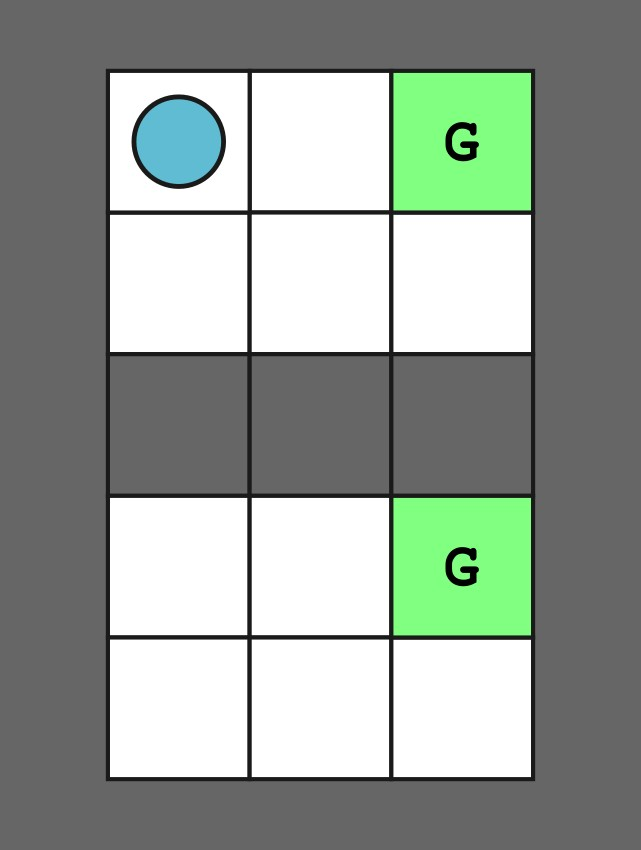
\includegraphics[width=\linewidth]{Figures/grid world.jpg}
        \caption{Grid World}
        \label{fig:grid_world}
    \end{subfigure}
    \hfill
    \begin{subfigure}{0.6\textwidth}
        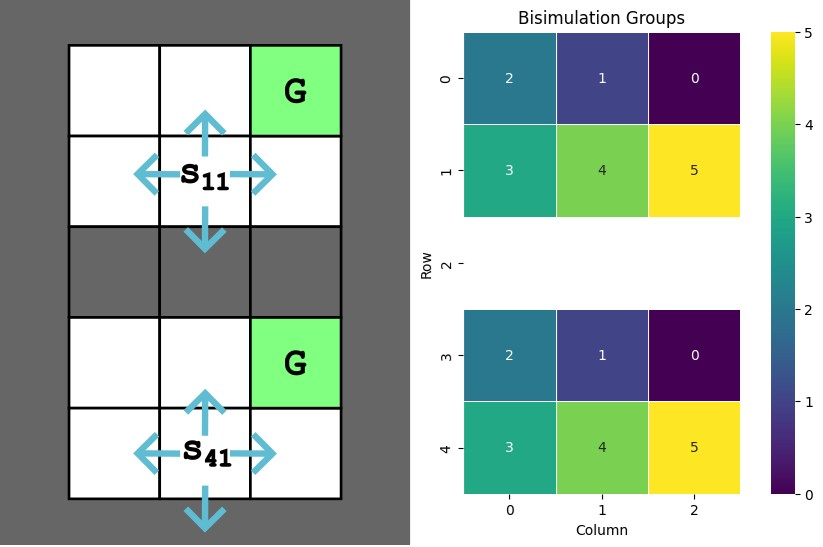
\includegraphics[width=\linewidth]{Figures/bisimulation.jpg}
        \caption{Bisimulation}
        \label{fig:bisimulation_grid_world}
    \end{subfigure}
    \caption[Bisimulation in Grid World]{\textbf{Bisimulation in Grid World}. A basic Grid World illustrating the process of obtaining the largest bisimulation $\sim$, showing the agent (sky blue circle), goals (green G square), transitions, actions, and reward structures, demonstrating how bisimulation captures behavioral similar states into groups of equivalence classes.}

    \label{fig:outdated_priorities}
\end{figure}


However, in reinforcement learning, we are generally more interested in complex behaviors (e.g., high-dimensional states) rather than just symmetrical behaviors. We will progressively analyze more complex behaviors. For now, we start by opening a small passage between the two rooms. When a passage is introduced, the equivalence classes collapse to the identity relation, a trivial solution that is not useful in practice (see Figure \ref{fig:bisimulation_collapse}). This occurs because, as mentioned earlier, bisimulation is a very strong theoretical assumption that requires exact matching of rewards and transitions, which is often challenging to achieve in practice.


% In consequence, the on-policy bisimulation (Definition \ref{def:on-policy-bisimulation}) can be used to only focus on the transition and reward given by the policy action. Notice in the deterministic case, our Grid World, the Equation \ref{eq:on_policy_reward_transition} is reduced too
% \begin{equation}
% \begin{aligned}
% \textbf{Given } a & = \pi(x), \\
% r_x^\pi & = r_x^a \\
% \forall C \in \mathcal{S}_{B^\pi}, \mathcal{P}_x^\pi(C) & = \sum_{x^{\prime} \in C} P_x^a( x^{\prime})
% \end{aligned}
% \end{equation}
% In consequence, it easily to verified that the properties are satisfied, we only have to check one reward and one transition per state in order to hold the reward and transition equivalence properties, and obtain the largest on-policy bisimulation relation $\sim^\pi$. The results are show in the Figure \ref{fig:on_policy_bisimulation}, where we can notice that the on-policy bisimulation effectively reduces the initial MDP of 13 states to and MDP of 4 states. Recall that this method requires to have knowledge of the policy at hand; to showcase the nature of the on-policy bisimulation in its optimal case, we used the optimal policy $\pi^*$ obtained with a value iteration algorithm \cite{sutton2018reinforcement}, but in practice an online policy could be taken into account.

Consequently, the on-policy bisimulation (Definition \ref{def:on-policy-bisimulation}) can be used to focus only on the transitions and rewards determined by a given policy. Notice that, in the deterministic case of our Grid World, Equation \ref{eq:on_policy_reward_transition} simplifies to:

\begin{equation}
\begin{aligned}
\textbf{Given } a &= \pi(x), \\
r_x^\pi &= r_x^a, \\
\forall C \in \mathcal{S}_{B^\pi}, \quad \mathcal{P}_x^\pi(C) &= \sum_{x^{\prime} \in C} P_x^a(x^{\prime}).
\end{aligned}
\end{equation}

Thus, it is easy to verify that the properties are satisfied; we only need to check one reward and one transition per state to ensure the reward and transition equivalence properties hold, allowing us to obtain the largest on-policy bisimulation relation, denoted as $\sim^\pi$. Figure \ref{fig:on_policy_bisimulation} illustrated how the on-policy bisimulation effectively reduces the initial MDP of 13 states to an MDP of 4 states. Note that this method requires knowledge of the policy being used; to demonstrate the on-policy bisimulation in its optimal case, we employed the optimal policy $\pi^*$ obtained using a value iteration algorithm \cite{sutton2018reinforcement}. However, in practice, an online policy could also be considered.

\begin{figure}[h]
    \centering
    \begin{subfigure}{0.45\textwidth}
    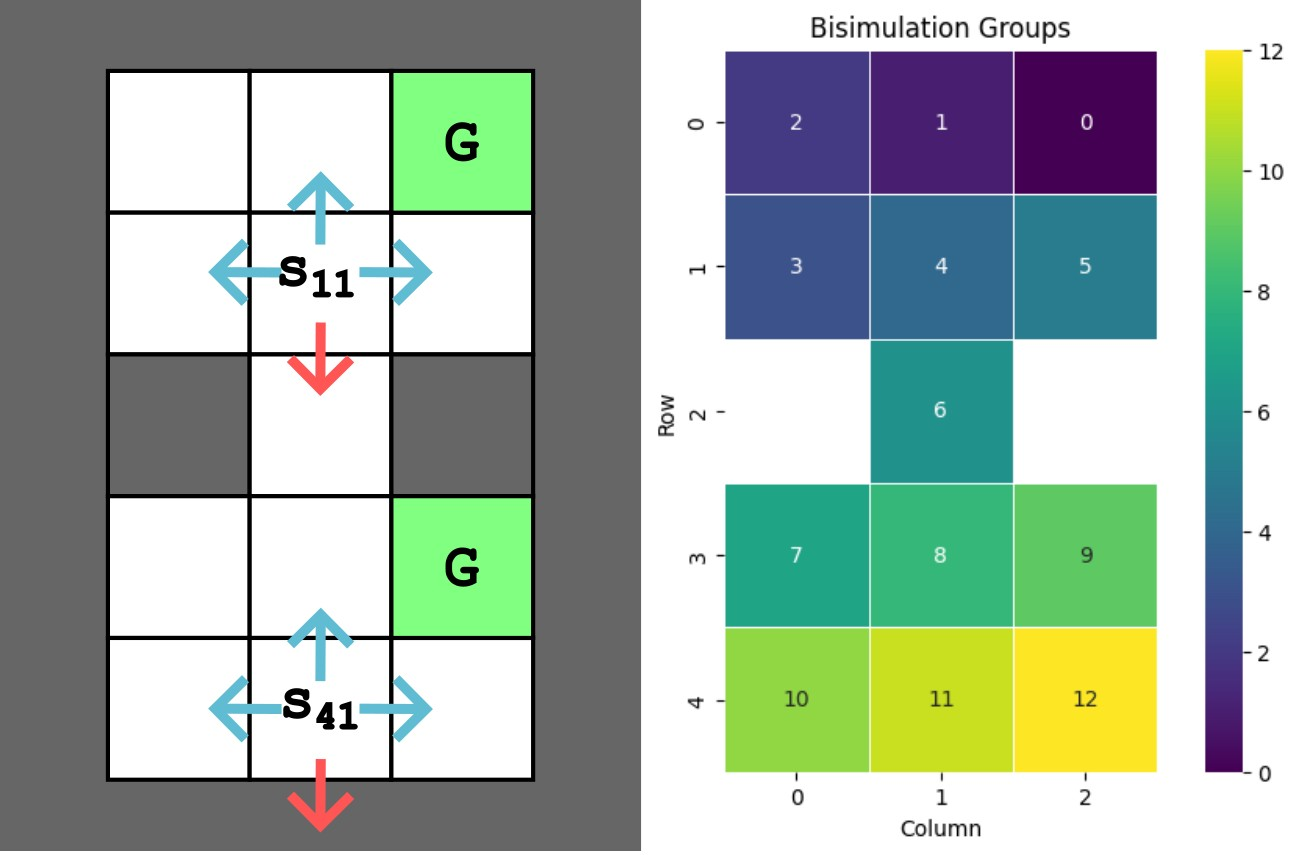
\includegraphics[width=\linewidth]{Figures/bisimulation_passage.jpg}
        \caption{Bisimulation Collapse}
        \label{fig:bisimulation_collapse}
    \end{subfigure}
    \hfill
    \begin{subfigure}{0.45\textwidth}
        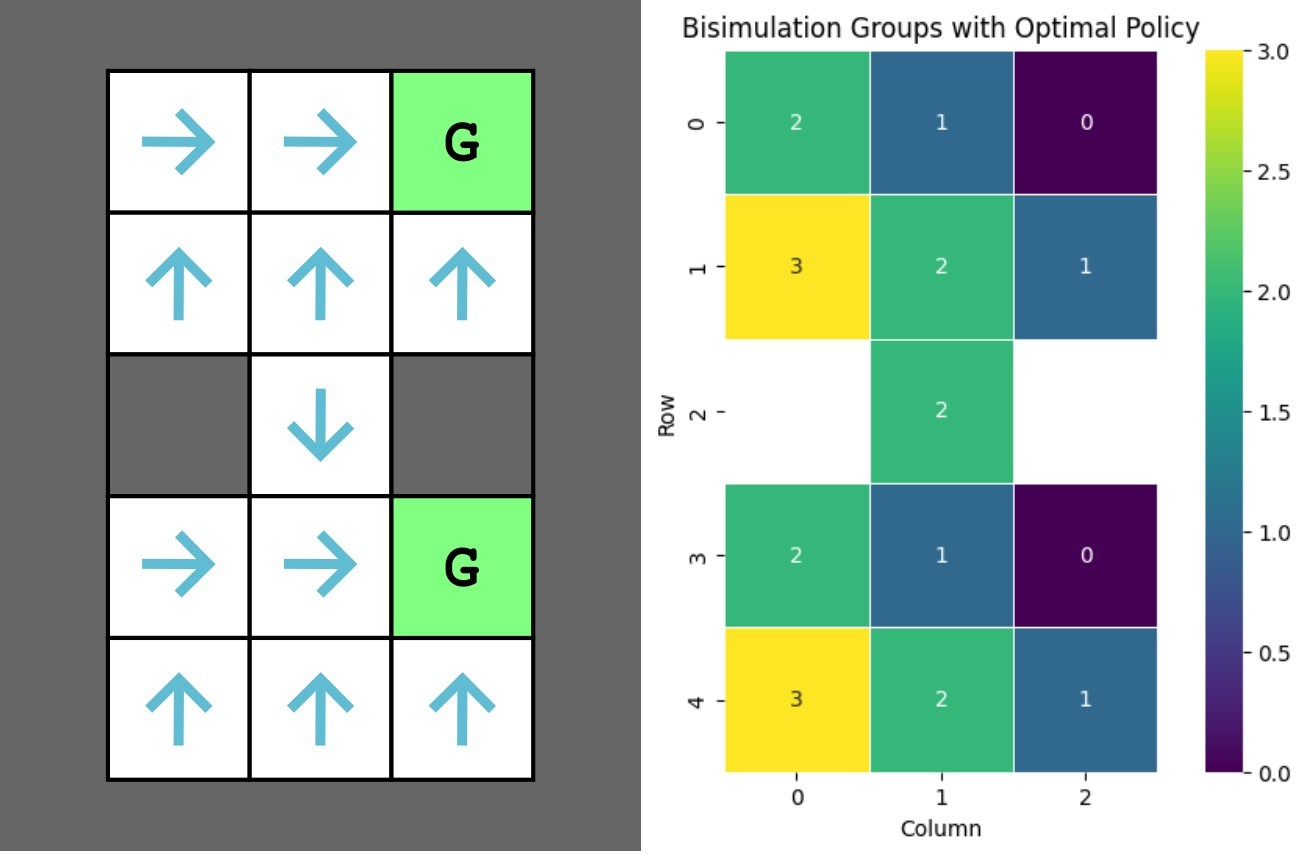
\includegraphics[width=\linewidth]{Figures/on_policy_bisimulation.jpg}
        \caption{On-policy Bisimulation}
        \label{fig:on_policy_bisimulation}
    \end{subfigure}
    \caption[Bisimulation Collapse and On-Policy Bisimulation]{\textbf{Bisimulation Collapse and On-Policy Bisimulation.} (a) Bisimulation collapse caused by the opening of a passage, violating the transitions equivalence between pairs of states, e.g. $s_{11}$, $s_{41}$. (b) A solution provided by on-policy bisimulation, satisfying reward and transition equivalence only for the given policy (denoted by sky blue arrows).}
\end{figure}

% While these groups clearly capture the behavioral similarity of states in the Markov Chain induce by the given policy, they still are not useful in practice for RL, where we are normally estimating things from data, and the calculation of equivalence relation are quite sensitive to infinitesimal variations. In such , we are more interested in provide a notion of behavioral distance from every state vs all the others. The on-policy bisimulation metric in Definition \ref{} provides us the means to do that. Specifically, in our Grid Word, according to Castro \cite{castro2020scalable}, it is possible to reduce the on-policy bisimulation operator to the following operator because our environment is deterministic

While these groups clearly capture the behavioral similarity of states in the Markov chain induced by the given policy, they are still not practical for reinforcement learning, where we commonly estimate values from data, and the calculation of equivalence relations can be highly sensitive to infinitesimal variations. Instead, we are more interested in providing a smoother equivalence notion with the use of behavioral distances from every state to all others. The on-policy bisimulation metric in Definition \ref{def:on_policy_bisimulation_metric} provide us the means to achieve this. Specifically, the deterministic nature of the Grid World allow us to reduce the on-policy bisimulation operator to the operator bellow according to Castro \cite{castro2020scalable}.

\begin{equation}
    \label{eq:deterministic_on_policy_bisimulation_metric}
    T^\pi_k(d)(x, y) = |r^\pi_x - r^\pi_{y}| + \gamma d(x',y') 
\end{equation}

where $x' = \mathcal{N}(x,\pi(x))$ corresponds to the next state given the state $x$ and the action taken by the current policy $\pi(x)$; in other words, $\mathcal{N}$ is a function that deterministically selects the next state with $P(\mathcal{N}(s,\pi(S)) = 1$.

Given that the on-policy operator $T^\pi_k(d)$ is a contraction mapping that converges to a fixed point \(d^\pi_\sim\), we can leverage the recurrence relation over \(d\) in Equation \ref{eq:deterministic_on_policy_bisimulation_metric} to obtain the \textbf{exact on-policy bisimulation metric} through an iterative application of the operator, starting from an initial estimate \(d_0\).

$$d_0 \rightarrow T^\pi_1(d_0) = d_1 \rightarrow T^\pi_2(d_1) = d_2 \cdots \rightarrow d^\pi_\sim$$

Specifically, we can initialize \(d_0\) in a tabular form as a matrix of full zeros, where each cell corresponds to a pair of states in the environment (see Figure \ref{fig:iterative_process}). The updates are then made using a dynamic programming approach by repeatedly applying the following rule:
\begin{equation}
    d_n(x,y) \leftarrow |r_x^a - r_y^a| + \gamma d_{n-1}(x',y'),
\end{equation}
where \(x'\) and \(y'\) are the next states from taking action \(a\) in states \(x\) and \(y\), respectively.

\begin{figure}[h]
    \centering
    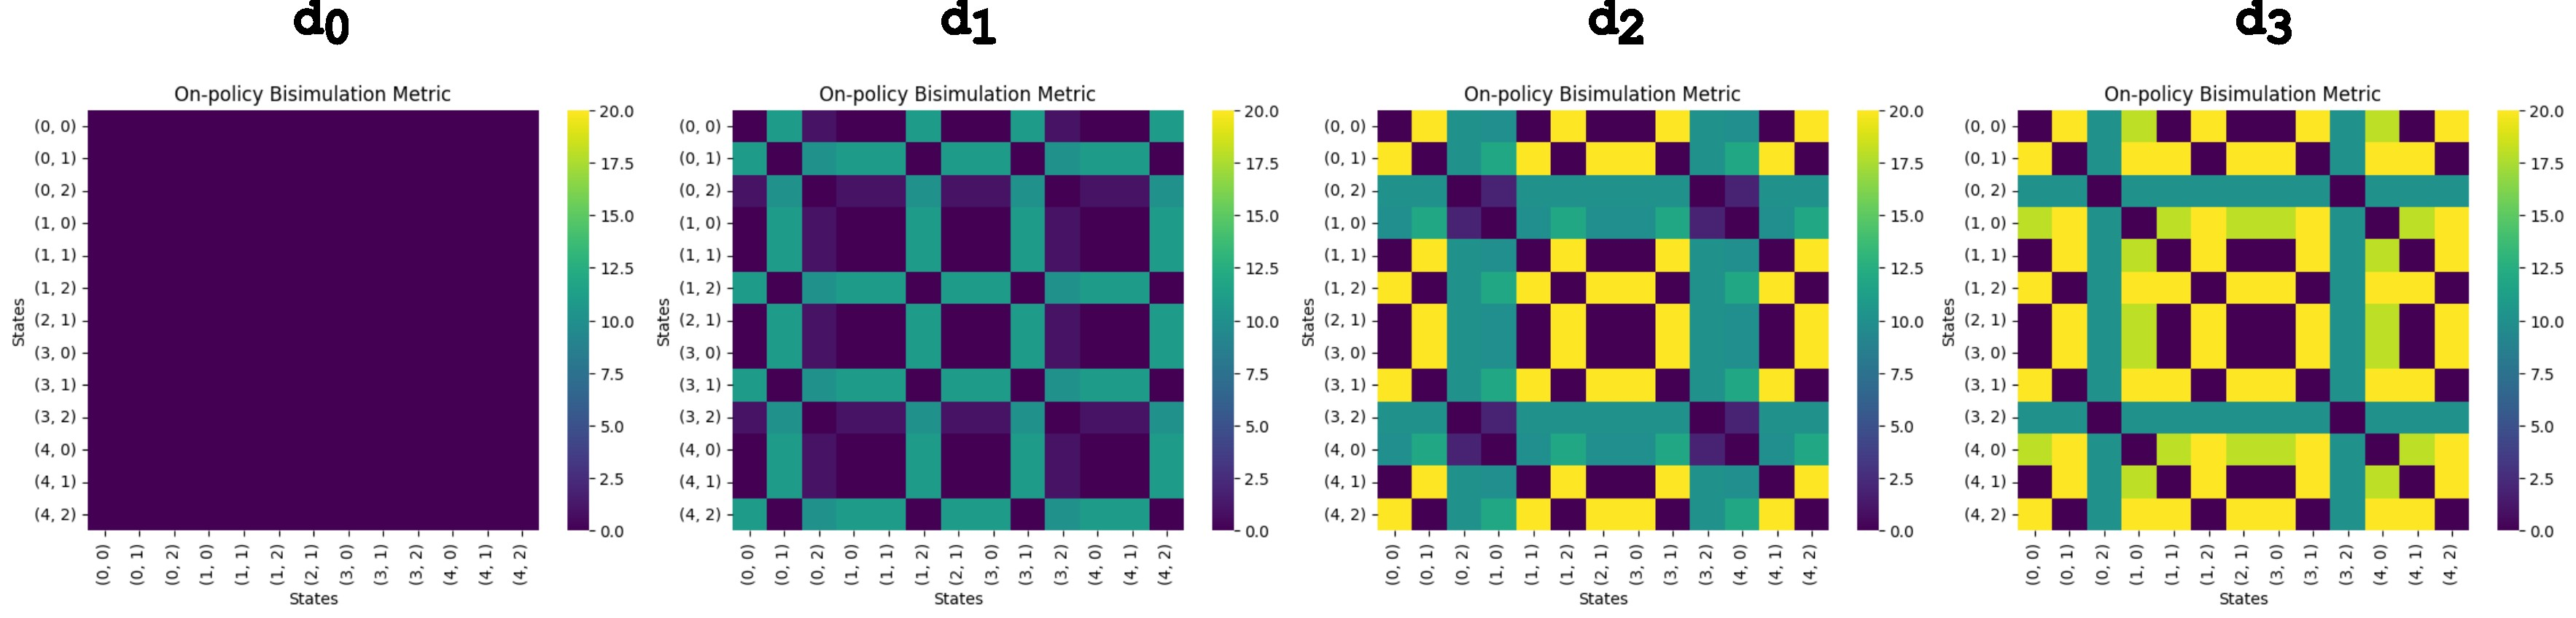
\includegraphics[width=1.\linewidth]{Figures/iterative process.jpg}
    \caption[Recursive On-policy Bisimulation Operator]{\textbf{Recursive On-Policy Bisimulation Operator.} Exact on-policy bisimulation metric through recursive updates of an initial estimate \(d_0\) that converges to \(d_3 = d_\sim^\pi\).}
    \label{fig:iterative_process}
\end{figure}

By applying a Multidimensional Scaling algorithm to the final fixed point distances \(d^\pi_\sim\), we can obtain an approximation of the states in a 2D plane (see Figure \ref{fig:clustering}), effectively clustering states with similar behaviors under a soft notion of distance. It is evident that the on-policy bisimulation distance tends to place behaviorally similar states close together and behaviorally dissimilar states further apart.

\begin{figure}[h]
    \centering
    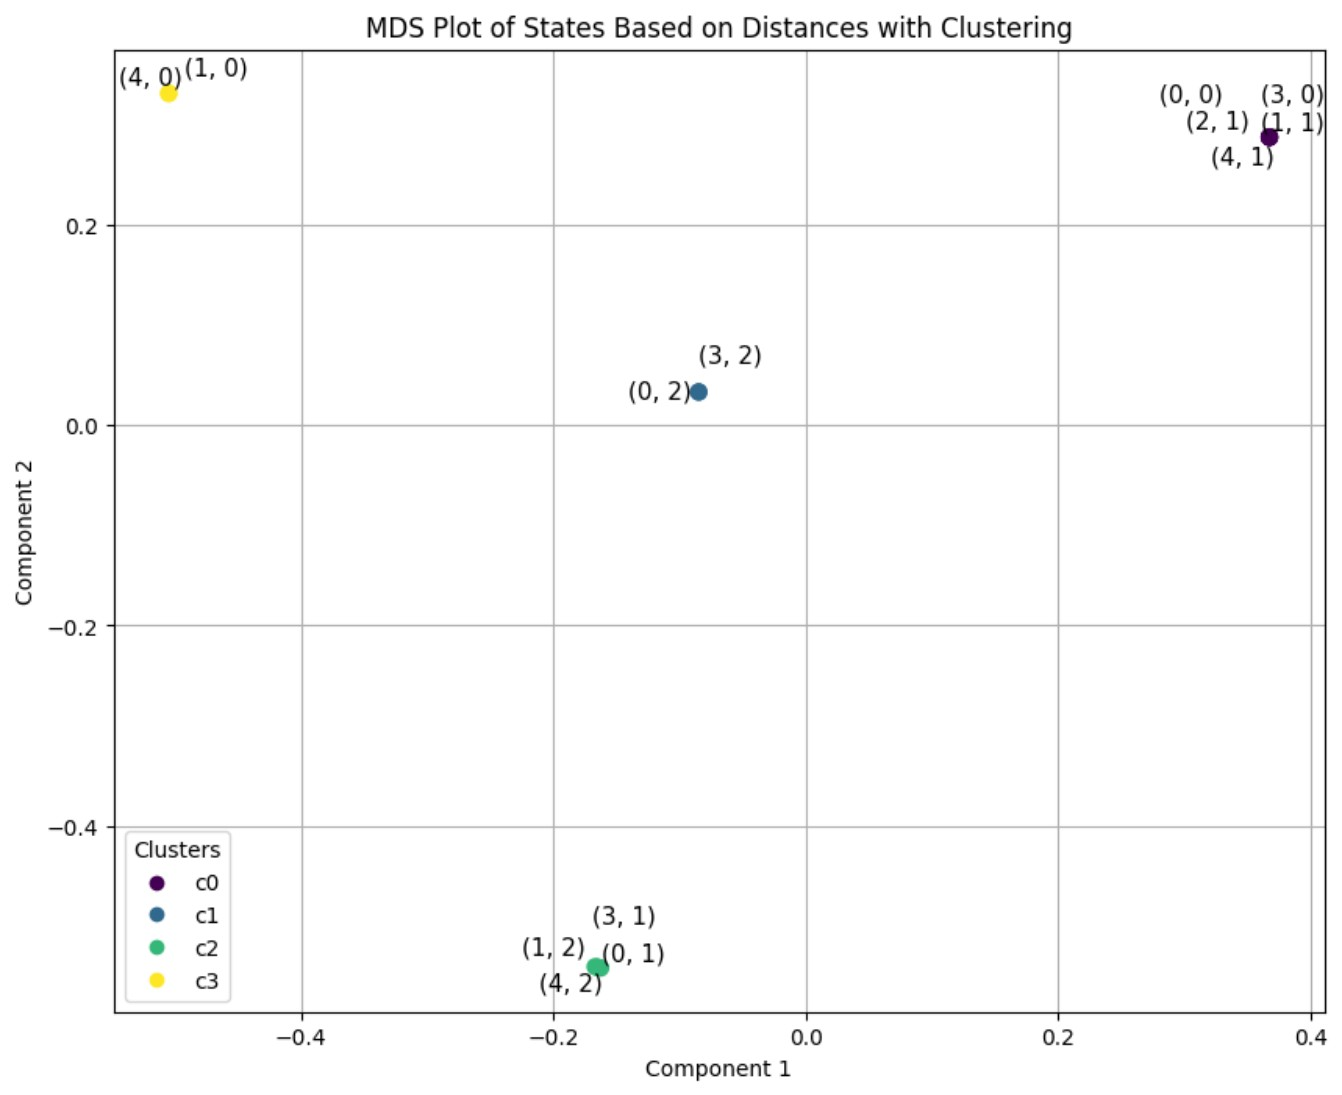
\includegraphics[width=0.9\linewidth]{Figures/clustering.jpg}
    \caption[Multidimensional Scaling of On-policy Bisimulation Distances]{\textbf{Multidimensional Scaling of On-Policy Bisimulation Distances.} The MDS algorithm is applied to on-policy bisimulation distances, revealing clusters of states separated according to the computed distances.}
    \label{fig:clustering}
\end{figure}


% The \textbf{Reward Equivalence}, corresponding to the Equation \ref{eq:reward_equivalence}, corresponds to analyze all the possible transitions between state $s_i$ and $s_j$

In the current work, we are interested in exploring these behaviors in terms of the experiences stored in the experience replay. Note that an experience tuple is defined as \(e_t = (s_t, a_t, r_t, s_{t+1})\). It is evident that experiences with a higher on-policy bisimulation distance between \(s_t\) and \(s_{t+1}\) are likely to be more informative (or 'surprising') than transitions between behaviorally similar states (see Figure \ref{}). By prioritizing transitions with greater behavioral differences, we encourage more diversity in the sampling process. This is the main idea behind our approach. Our method leverages these behavioral distance notions to promote more diverse sampling in the experience replay.

%\subsection{On-policy MICO metric justification}
\section{Bisimulation Prioritized Experience Replay}

The previous example provides a method to calculate the on-policy bisimulation metric in deterministic MDPs and environments with a few states. However, in practice, we often encounter more complex environments with high-dimensional representations (e.g., pixels), where calculating on-policy bisimulation metrics in a tabular form becomes intractable.

To address these challenges, we employ an indirect approach to approximate these bisimulation metrics within the RL loop. Specifically, works by Zhang et al. \cite{zhang2020learning} and Castro et al. \cite{castro2021mico} have demonstrated that it is more effective and general to obtain a bisimulation metric as part of the online learning of state abstractions. In the following, we will detail the specific method for learning these abstractions and how this approach allows us to approximate the metric on the fly.

\subsection{Learning State Abstractions}

The present work employs a surrogate on-policy bisimulation metric known as the MICO metric \cite{castro2021mico} (see Definition \ref{def:mico_operator}). The MICo metric substitutes the Kantorovich distance $\mathcal{W}_d$ calculation with the independent coupling. For reference, we restate the operator equation here:
$$
\label{eq:mico_operator}
    T^\pi_M(U)(x, y) = |r^\pi_{x} - r^\pi_{y}| + \gamma \mathbb{E}_{x'\sim P_x^\pi, y'\sim P_y^\pi}\left[U(x',y') \right]
$$

% , where the first term corresponds to the reward equivalence difference, and the second corresponds to the independent coupling.

The MICo operator is used to learn a parameterized state abstraction \(\phi_\omega(x) : \mathcal{S} \to \mathcal{S}_\phi\) (parameterized by \(\omega\)), which maps a true environmental state (e.g., pixels) to a lower-dimensional latent representation. The goal is to position these representations in such a way that a chosen parameterized distance $U_\omega(x,y)$ (e.g., Euclidean, cosine) coincides with the MICo distance in the latent space (see Figure \ref{}). However, since the MICo distance is a diffuse metric (see Definition \ref{def:diffuse_metric}), the parameterized distance must ensure positive self-distances. To achieve this, the following parameterized distance function was proposed in \cite{castro2021mico} for any \(x, y \in \mathcal{S}\):
\begin{equation}
    U^\pi(x, y) \approx U_\omega(x, y):=\frac{\left\|\phi_\omega(x)\right\|_2^2+\left\|\phi_\omega(y)\right\|_2^2}{2}+\beta \theta\left(\phi_\omega(x), \phi_\omega(y)\right)
\end{equation}

where the first term ensures positive self-distances\footnote{In theory, the second term can be any other notion of distance, such as the euclidean distance. However, empirical results from MICo\cite{castro2021mico} have shown that the angular distance provides greater numerical stability.}, $\phi_\omega(x), \phi_\omega(y)$ corresponds to the abstract representations, $\theta\left(\phi_\omega(x), \phi_\omega(y)\right)$ is the angle between vectors $\phi_\omega(x)$ and $\phi_\omega(y)$, and $\beta$ is an hyperparameter.

Consequently, the recursive nature of the operator \(T_M^\pi(U)(x,y)\) is used to define a loss function, which works similarly to the Bellman recurrence process in DQN. In this approach, a target is defined, and we aim to approximate this target with a online estimate. Specifically, in our case, the loss function measures the difference between a learning target MICo metric\footnote{\(U_{\bar{\omega}}\) is an unbiased estimator of the independent coupling.} \(T_{\bar{\omega}}^U\) and the online MICo metric \(U_\omega\), as 

\begin{equation}
\label{eq:mico_loss}
    \mathcal{L}_{\mathrm{MICo}}(\omega)=\mathbb{E}_{\left\langle x, r_x, x^{\prime}\right\rangle,\left\langle y, r_y, y^{\prime}\right\rangle}\left[\left(T_{\bar{\omega}}^U\left(r_x, x^{\prime}, r_y, y^{\prime}\right)-U_\omega(x, y)\right)^2\right]
\end{equation}

\begin{equation}
    T_{\bar{\omega}}^U\left(r_x, x^{\prime}, r_y, y^{\prime}\right)=\left|r_x-r_y\right|+\gamma U_{\bar{\omega}}\left(x^{\prime}, y^{\prime}\right)
\end{equation}

where \(\bar{\omega}\) is a separate copy of the network parameters, synchronized with \(\omega\) at infrequent intervals, and the pairs of transitions \(\left\langle x, r_x, x^{\prime}\right\rangle\) and \(\left\langle y, r_y, y^{\prime}\right\rangle\) are sampled from the experience replay.\footnote{The actions are not considered in the experiences because we assume a fixed policy under the on-policy assumption.} \footnote{When distances are large, they can oversaturate the MICo loss, causing instability in gradient updates. Therefore, in practice, a Huber loss is employed to focus on small differences between states.}

The MICO learning can be integrated into any value-based agent by learning an estimate $Q_{\xi, \omega}(x, \cdot) = \psi_\xi(\phi_\omega(x))$, where $\phi_\omega(x)$ corresponds to the representation of state $x$, and $\psi_\xi$ corresponds to the value approximator. This work specifically focuses on the DQN algorithm (see Section \ref{sec:dqn}), where the $Q_{\xi, \omega}$ corresponds to the Q-values. In this scenario, the MICO loss $\mathcal{L}_{\text{TD}}$ is combined with the temporal-difference loss $\mathcal{L}_{\text{MICo}}$ as 
\begin{equation}
    \mathcal{L}_\alpha(\xi, \omega) = (1 - \alpha)\mathcal{L}_{\text{TD}}(\xi, \omega) + \alpha \mathcal{L}_{\text{MICo}}(\omega)
\end{equation}
, where $\alpha \in (0, 1)$. 
Figure \ref{} illustrates the network architecture used for learning, showing that the MICo loss is applied directly after the convolution layers and used to calculate the total loss $\mathcal{L}_\alpha$. Note that the same parameters $\omega$ are shared for both losses and both inputs, without the need for additional parameters.


% Additionally, notice the network are identical for both only the inputs are different. In such way, no extract parameters are used to learn the representation

Although the MICo loss $\mathcal{L}_{\text{MICo}}$ requires pairs of transitions $\left\langle x, r_x, x^{\prime}\right\rangle$ and $\left\langle y, r_y, y^{\prime}\right\rangle$, in practice, transitions are not sampled as pairs; we only have access to a mini-batch of unpaired transitions, necessitating a method to pair them. To address this issue, a \textbf{squarify} method \cite{castro2020scalable} was proposed to construct pairs of transitions by pairing each transition with all others within the current mini-batch and then calculating the MICo loss. Figure \ref{} illustrates how this squarify process works.

% Then, the metric is used as part of a loss function to learn state abstractions.  Specifically, in this work, an encoder will map high-dimensional states (e.g., frames from an RL environment) into a lower-dimensional latent space, such that behaviorally similar states are kept closer together and behaviorally dissimilar states are kept farther apart in the latent space.

\subsection{Priority Strategies}


In the following, we propose our method, \textbf{Bisimulation Prioritized Experience Replay (BPER)}, along with \textbf{two strategies} for calculating these priorities on the fly, based on certain hypotheses. As mentioned before, the MICo metric is approximated online as part of the state abstraction learning process, so that it is enough to use $U_\omega$ to calculate a MICo distance between two states and update the priorities accordingly.

Another possible option for calculating the distance online is to use the target distance \(T^U_{\bar{\omega}}\), which uses the corresponding rewards difference. However, since the metric will eventually converge to a fixed point, it is sufficient and more convenient to use \(U_\omega\), as this approach does not require incorporating rewards into its calculation.

% \subsubsection{Strategy 1: Current vs Next (BPERcn)}

\begin{strategy}[\textbf{Current vs Next: BPERcn}]
Consider a current minibatch \(B \subset \mathcal{E}\), $|B| = k$, containing transition experiences \(e_i = (s_i, r_i, a_i, s_{i+1})\). Each transition can be associated with a distance \(U_\omega(s_i, s_{i+1})\), which effectively quantifies how behaviorally different the \textbf{current state} \(s_i\) is compared to the \textbf{next state} \(s_{i+1}\). Consequently, the re-weighted priority is calculated as follows:

\begin{equation}
    p_i = (1 - \mu) |\delta_i| + \mu U_\omega(s_i, s_{i+1}) + \epsilon,
\end{equation}

where \(\delta_i\) corresponds to the TD-error of the experience, \(\mu \in [0,1)\) controls the balance between the TD-error and the bisimulation distance, and \(\epsilon\) is a small positive constant to ensure that experiences are revisited even when the weighted priority is equal zero.
\end{strategy}

The distance \(U_\omega(s_i, s_{i+1})\) serves as an indicator of a 'surprising' transition, suggesting that transitions with larger distances are more informative and likely to contribute to greater learning progress. While using TD-error as an standalone method could potentially overemphasize some transitions, leading to a loss of diversity \cite{schaul2015prioritized},\cite{pan2022understanding},\cite{fedus2020revisiting}, our method consistently encourages diversity in the experiences by reweighting the TD-error, regulated by a parameter $\eta \in [0,1)$.

Similar to a proportional prioritization in PER \cite{schaul2015prioritized} (see Section \ref{sec:per}), the sampling probability for an experience $e_i$ is given by $P(t) = \frac{p_t^\alpha}{\sum_k p_k^\alpha}$, where $\alpha$ controls the degree of prioritization. Additionally, the weighted importance sampling for unbiased updates is computed as $w_i = \left(\frac{1}{N} \cdot \frac{1}{P(i)} \right)^\beta$, followed by a normalization step $\frac{1}{\max_k w_k}$. In practice, a sum tree data structure is used to optimize the sampling procedure.
% \subsubsection{Strategy 2: All vs All (BPERaa)}

Strategy 1 provides a theoretical valid method to characterize the priority of transition based on a behavioral distance between the current and next state. However, in practice, the trajectories may overlap significantly, resulting in \textbf{overlapping states distributions} with highly similar behaviors. Additionally, since the bisimulation is approximated online, there are sources of variability in the approximation until reaching the convergence point. These issues can trigger trajectories with many similar distances between current and next states (see Figure \ref{}), with only a few behavioral different states appearing after long rollouts; resulting in scarce high-priority transitions, and consequently affecting the effectiveness of prioritization technique. To address these issues, the following empirical solution is proposed. 

\begin{strategy}[\textbf{All vs All: BPERaa}]
Consider a minibatch $B \subset \mathcal{E}$, $|B| = k$, with transition experiences $e_i = (s_i, r_i, a_i, s_{i+1})$. Each transition $e_i$ can be associated with a relative bisimulation distance

\begin{equation}
    U^B_\omega(s_i) = \sum_{i=1}^k U_\omega(s_i, s_k), \quad \forall e_k = (s_k, r_k, a_k, s_{k+1}) \in B
\end{equation}

Consequently, the re-weighted priority will be calculated as follows

\begin{equation}
    p_i = (1 - \mu) |\delta_i| + \mu U^B_\omega(s_i) + \epsilon
\end{equation}
where \(\delta_i\) corresponds to the TD-error of the experience, \(\mu \in [0,1)\) controls the balance between the TD-error and the bisimulation distance, and \(\epsilon\) is a small positive constant to ensure that experiences are revisited even when the weighted priority is equal zero.
\end{strategy}


Although the current states from different transitions are not directly connected by a valid transition, the bisimulation metric allows us to measure behavioral dissimilarity between all states in the environment. This enables the calculation of a behavioral distance relative to the current minibatch by computing the mean distance between each current state and all other states in the minibatch (see Figure \ref{}). This relative distance serves as a smoother indicator of how behaviorally dissimilar one initial state is compared to the others, indicating 'surprising' or more informative transitions. Figure \ref{} illustrates how the initial states of all transitions in the minibatch are positioned in the latent space, with more behaviorally distinct states placed farther apart. In practice, we use the squarify method, along with reshaping and averaging operations, to compute these distances on the fly. Similar as before, the $\alpha$-priority, weighted importance sampling and sum tree data structure are used for the sampling procedure.

Algorithm \ref{algorithm:dqn_bper} illustrates the entire prioritizing process, highlighting the modifications made to the original and prioritized version. Similar to the PER method the priorities are only updated for the current sampled mini batch to maintain computational efficiency. Notice the algorithm depicts the procedure for Strategy 1 (BPERcn). Strategy 2 (BPERaa) requires a minor replacement in line 19, where \(U_\omega(s_i, s_{i+1})\) should be replaced with \(U^B_\omega(s_i)\). An additional algorithm illustrating only MICo learning with DQN, without BPER, is provided in Appendix \ref{} for reference.

\begin{algorithm}
\caption{DQN with Bisimulation Prioritized Experience Replay (BPERcn)}
\label{algorithm:dqn_bper}
\begin{algorithmic}[1]
\State \textbf{Input:} minibatch $k$, step-size $\eta$, replay period $K$ and size $N$, exponents $\alpha$ and $\beta$, budget $T$ (total steps), priority weigh $\mu$.
\State \textbf{Initialize} action-value function $Q$ with random weights $\xi$, $\omega$
\State \textbf{Initialize} target action-value function $Q^-$ with weights $\{\bar{\xi},\bar{\omega}\} \leftarrow \{\xi, \omega\}$
\State \textbf{Initialize} replay memory $\mathcal{D} = \emptyset$ with capacity $N$, $p_1 = 1$ (inital priority) %$\Delta_{\{\xi, \omega\}} = 0$, $\Delta_\omega = 0$, $p_1 = 1$
% \State Observe $s_0$ and choose $a_0 \sim \pi^\epsilon_\theta(s_0)$ 
\For{$t = 1$ to $T$}
    \State Observe $s_t$
    \State Choose action $a_t \sim \pi^\epsilon_\theta(s_t)$
    \State Execute action $a_t$ and observe $r_t$ and $s_{t+1}$
    \State Store transition $(s_t, a_t, r_t, s_{t+1})$ in $\mathcal{D}$ with maximal priority $p_t = \max_{i < t} p_i$
    \If{$t \equiv 0 \mod K$}
        % \For{$j = 1$ to $k$}
        \State Sample minibatch $B$ of transitions $e_j$ with probability $P(j) = \frac{p_j^\alpha}{\sum_i p_i^\alpha}$    
        \State Compute importance-sampling weight $w_j = \left( N \cdot P(j) \right)^{-\beta} / \max_i w_i$
        \State Set $y_j = 
        \begin{cases} 
            r_j & \text{for terminal } s_{j+1}\\
            r_j + \gamma \max_{a'} Q^-(s_{j+1}, a'; \{\bar{\xi},\bar{\omega}\}) & \text{otherwise}
        \end{cases}$
        \State Compute TD-error $\delta_j = y_j - Q(s_{j}, a_{j}; \{\xi, \omega\})$, and loss $\mathcal{L}_{\text{TD}} = \delta_j^2 $
        \State Squarify minibatch $B$ to get transition pairs $\left\langle x, r_x, x^{\prime}\right\rangle,\left\langle y, r_y, y^{\prime}\right\rangle$ 
        \State Compute MICo loss $\mathcal{L}_{\text{MICo}} = \left(T_{\bar{\omega}}^U\left(r_x, x^{\prime}, r_y, y^{\prime}\right)-U_\omega(x, y)\right)^2$
        \State Compute total loss $\mathcal{L}_\alpha(\xi, \omega) = (1 - \alpha) \mathcal{L}_{\text{TD}}(\xi, \omega) + \alpha \mathcal{L}_{\text{MICo}}(\omega)$
        \State Perform a gradient descent step on $\mathcal{L}_\alpha(\xi, \omega)$, weighting the updates by $w_j$
        \State Update transition priority $p_j \leftarrow (1 - \mu) |\delta_j| + \mu U_\omega(s_j,s_{j+1}) + \epsilon$
        \State Every C optimizing steps update $\{\bar{\xi},\bar{\omega}\} \leftarrow \{\xi, \omega\}$
        

        
        % \State Accumulate weight-change $\Delta_{\{\xi, \omega\}} \leftarrow \Delta_{\{\xi, \omega\}} + w_j \cdot \delta_j \cdot \nabla_\theta Q(s_{j}, a_{j})$
        % \State Compute bisimulation distance error $\sigma_j = T_{\bar{\omega}}^U\left(r_x, x^{\prime}, r_y, y^{\prime}\right)-U_\omega(x, y)$
        %  \State Accumulate weight-change $\Delta_{\omega} \leftarrow \Delta_{\omega} + w_j \cdot \sigma_j \cdot \nabla_\omega U_\omega(s_{i}, a_{j})$   

        % \EndFor
        % \State Update weights $\theta \leftarrow \theta + \eta \cdot \Delta$, reset $\Delta = 0$
    \EndIf
\EndFor
\end{algorithmic}
\end{algorithm}

\section{Experimentation Setup}

% \subsection{Experiments and Environments}
The proposed method will be tested in two setups: 1) 31-state Grid Worlds illustrated in Figure \ref{fig:behavioral_similarity}; similar to those environment in the works of Pan et al. \cite{pan2022understanding} and Castro \cite{castro2020scalable}, where calculating the bisimulation metrics is relatively straightforward; and 2) the Classic Control benchmark suite\footnote{Classic Control benchmark: \href{https://www.gymlibrary.dev/environments/classic_control/}{https://www.gymlibrary.dev/environments/classic\_control/}}, and the Lunar Lander from the Box2D suite\footnote{Box2D suit benchmark: \href{https://gymnasium.farama.org/environments/box2d/}{https://gymnasium.farama.org/environments/box2d/}}. In these setups, states will be \textbf{partially observable derived from pixels}, rather than full descriptive states.

The experiments aims to validate our proof of concept rather than test state-of-the-art results. Although the Grid Word is trained using pixels-based states, the underlying 31-state MDP enable us to measure evaluation metrics without high computational cost. Specifically, we will use the Grid World to evaluate our algorithm's performance on three key problems:

\begin{itemize}
    \item First, to evaluate the \textbf{task-agnostic sampling} problem, we examined how well the algorithm prioritizes behaviorally dissimilar states by showing distributions of priorities and behavioral similarities, similar to the experiments in Castro's work \cite{castro2020scalable}.

    \item Second, to evaluate the \textbf{outdated priorities} problem, we replicated the sampling distribution experiments from Pan et al.'s work \cite{pan2022understanding}. The purpose of this experiment is to assess how closely the priorities updated per minibatch align with the ideal case, where the priorities of the entire state space are updated at each time step. To measure this, we used two distance schemes proposed in Pan et al.'s work \cite{pan2022understanding}.

    Given the sampling distribution of priorities \(p_i(\cdot)\) from the experience buffer and the corresponding ideal distribution \(p_i^*(\cdot)\) (theoretically achieved when all state space priorities are updated at each time step\footnote{While the ideal distribution represents the best-case scenario, it is impractical to update all possible state priorities under the current policy at each step in practice.}), 1) the on-policy weighting is given by \(\sum_{j=1}^{31} w^\pi(s_j) | p_i(s_j) -p_i^*(s_j)|, i \in \{1,2\}\), and 2) the uniform weighting is \(\frac{1}{31} \sum_{j=1}^{31} | p_i(s_j) -p_i^*(s_j) |, i \in \{1,2\}\), where \(p_1\) corresponds to the PER method and \(p_2\) corresponds to the BPER method. A more detailed explanation of this procedure is provided in the Appendix \ref{}.
    
    \item Third, to evaluate \textbf{state space coverage}, we visually and quantitatively assessed the level of exploration per algorithm. We plotted the distribution of visited states in our Grid Worlds, similar to \cite{pan2022understanding}, and calculated the corresponding entropy of the state visitation distribution as $H(\mathcal{S}) = - \sum_{i=1}^{|\mathcal{S}|} p(s_i) \log p(s_i)$, where \(p(s_i)\) is the probability of visiting state \(s_i\), calculated as the ratio of visits to state \(s_i\) over the total number of visits to all states.
\end{itemize}


Finally, we performed standard test (time steps vs. episodic reward) to compare our algorithm's performance against standard ER and Prioritized ER in slightly more complex environments, such as: Cartpole, Mountain Car, Acrobot, and LunarLander, using pixel-based states. As many episodic reward results overlap, we decided to plot the \textbf{Episode Reward Gain} by comparing the methods PER, BPERaa, and BPERcn against two baselines: DQN and DQN + MICo. The Episode Reward Gain is calculated per episode as follows: \(\mathcal{R}^G(\tau) = \mathcal{R}_{\text{method}}(\tau) - \mathcal{R}_{\text{baseline}}(\tau)\), where \(\tau\) can correspond to trajectories of different lengths\footnote{To handle these differences, we use back and forward filling for NaN values in the episodic reward trajectory results.}. A positive Episode Reward Gain indicates an improvement over the baseline, while a negative value indicates underperformance compared to the baseline.

The RL algorithm used for all our experiments was DQN \cite{mnih2013playing}, with extensions added in a plug-in fashion while maintaining consistent hyperparameters across different environments and algorithms to ensure fair comparisons. For PER and MICo state-of-the-art hyper-parameters were used, extracted from the original papers, and only a sweep over the newly introduced hyperparameter \(\nu\) was conducted for the 31-state Grid World. A detailed explanation of the hyperparameters used is provided in Appendix \ref{}.

The algorithms were implemented using the TorchRL library\footnote{TorchRL: \href{https://pytorch.org/rl/stable/index.html}{https://pytorch.org/rl/stable/index.html}}. Specifically, the baseline DQN algorithm was taken from the SOTA implementations available at the \href{https://github.com/pytorch/rl/tree/main/sota-implementations/dqn}{TorchRL GitHub repository}, and the corresponding extensions (PER, MICo, MICo + BPER) were developed and added. The MICO extension was reproduced on TorchRL based on the original repository: \href{https://github.com/google-research/google-research/tree/master/mico}{Google Research MICO}. The experiments were executed on an RTX 4060 GPU with 8GB of memory. The algorithm is accessible through the university GitLab and a \href{https://github.com/ZosoV/final_project}{personal GitHub}.
% \subsection{TorchRL}



